%%%%%%%%%%%%%%%%%%%%%%%%%%%%%%%%%%%%%%%%%%%%%%%%%%%%%%%%%%%%%%%%%%%%%%%%%%%%%%%%%%%%%%%%%%%%%%%%%%%%%%%%%%%%%%%%%%%%%%%%%%%%%
\clearpage
\subsubsection*{AVA (Atomic Visual Action)}
\begin{figure}[!ht]
	\centering
	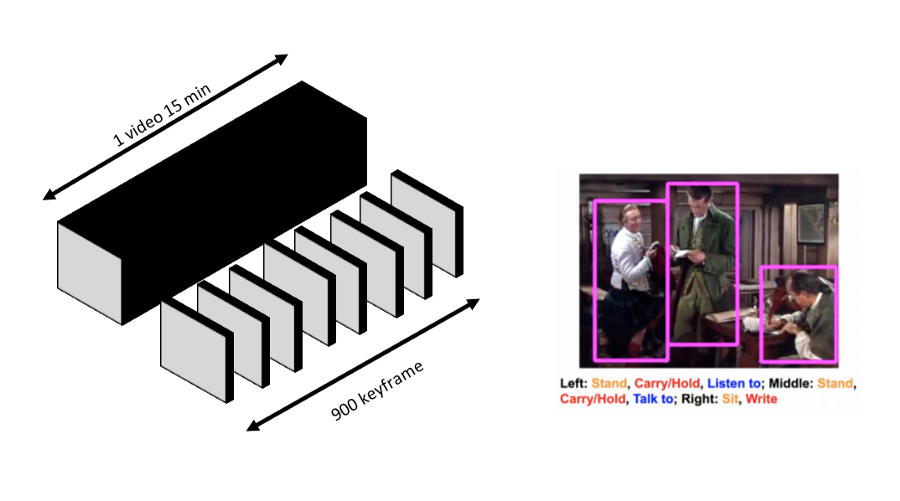
\includegraphics[width=1\textwidth]{chapter2/images/AVA.png}
		\caption{ด้านซ้าย แสดงการสุ่มตัวอย่าง (sampling)วิดีโอ เป็นคีย์เฟรม(keyframes) , ด้านขวา แสดงคีย์เฟรม (keyframes) ที่ถูก labels ซึ่งเป็น Multiple label annotation}
    	\label{fig:AVA}
\end{figure}
AVA คือ ชุดข้อมูลที่รวบรวมวิดิโอที่มีความยาว 15 นาทีและจะถูกแบ่งด้วยความถี่ 1 hz (900 keyframes) จากในหนังโดยยึดการกระทำของมนุษย์เป็นศูนย์กลาง เพื่อใช้สำหรับสร้างโมเดลที่เข้าใจกิจกรรมของมนุษย์ในวิดิโอว่ามนุษย์กำลังทำอะไรอยู่ ซึ่งข้อดีของ AVA คือ ชุดข้อมูลจะมีคำอธิบาย (label) เป็นแบบ multiple label (ในหนึ่งกรอบสี่เหลี่ยม (bounding box) สามารถมีคำอธิบายได้หลายคำอธิบาย) และคำอธิบายของ AVA (label) มีจำนวน 80 class สามารถแบ่งได้เป็น 3 หมวดหมู่คือ ท่าทาง (Pose) , ปฏิสัมพันธ์กับวัตถุ (Interaction with object) และ ปฏิสัมพันธ์กับบุคคล (Interaction with people) ซึ่งสามารถมีคำอธิบายได้มากสูงสุดถึง 7 คำอธิบาย

\subsubsection*{1. วิธีการรวบรวมข้อมูล}
\begin{figure}[!ht]
	\centering
	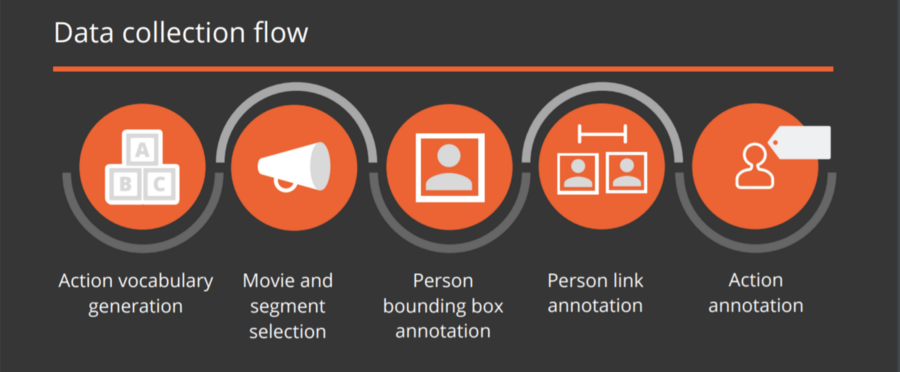
\includegraphics[width=1\textwidth]{chapter2/images/data_collection_ava.png}
		\caption{แสดงขั้นตอนการทำงานของการเก็บข้อมูลทำชุดข้อมูล}
    	\label{fig:data_collection_ava}
\end{figure}
ขั้นตอนการเก็บข้อมูลสำหรับการทำชุดข้อมูลมีขั้นตอนการทำ 5 ขั้น คือ
\begin{enumerate}
	\item การสร้างคำศัพท์การกระทำ (verb generation) จะมีหลัก 3 ข้อในการรวบรวมคำศัพท์ คือ
	\begin{enumerate}
		\item เก็บรวบรวมคำศัพท์ทั่วไปที่เกิดขึ้นในชีวิตประจำวัน
		\item จะต้องมีเอกลักษณ์ สามาถเห็นได้ชัดเจน เช่น การถือของ
		\item กำหนดรูปแบบของคำศัพท์ขึ้นมาและใช้ความรู้จากชุดข้อมูลอื่น ในการทำให้ได้ class การกระทำของมนุษย์ที่ครอบคลุมของชุดข้อมูล AVA
	\end{enumerate}
	\setlength\itemsep{-0.25em}
	\item  หนังและส่วนที่เลือกมาใช้ (Movie and segment selection)
วิดิโอที่ใช้ทำชุดข้อมูล AVA ทั้งหมดจะถูกนำมากจาก youtube โดยเริ่มจากการรวบรวมเอารายชื่อของนักแสดงที่มีชื่อเสียง ซึ่งจะมีความหลากหลายของเชื้อชาติรวมกันอยู่ ซึ่งวิดิโอที่ถูกคัดเลือกจะมีเกณฑ์ดังนี้ คือ
	\begin{enumerate}
		\item วิดิโอต้องอยู่ในหมวด หนัง และ ละครโทรทัศน์
		\item จะต้องมีความยาวมากกว่า 30 นาที
		\item อัพโหลดเป็นเวลาอย่างน้อย 1 ปี
		\item มียอดวิวคนดูมากกว่า 1000 วิว
		\item ละเว้นวิดิโอบางประเภท เช่น ขาว-ดำ , ความละเอียดต่ำ , การ์ตูน , วิดิโอเกม
		\item ในการเลือกวิดิโอที่มีข้อจำกัดจะต้องมีวิธีการเลือก คือ 
		\begin{enumerate}
			\item ไม่ทำการกรองวิดิโอออกด้วย action keywords 
			\item ไม่ทำให้เป็น uniform label distribution 
			\item เลือกแค่ส่วนหนึ่งของหนัง คือ ช่วงนาทีที่ 15 - 30 เนื่องจากต้องการที่จะข้ามส่วนต้นของหนัง ซึ่งอาจเป็น ตัวอย่างของหนัง หรือ โฆษณา
		\end{enumerate}	
	\end{enumerate}
	\setlength\itemsep{-0.25em}
	\item  การตีกรอบบุคคลที่อยู่ภายในภาพ(Person bounding box annotation) ประกอบด้วย 2 ขั้นตอน
	\begin{enumerate}
		\item สร้างกรอบสี่เหลี่ยม (bounding boxes) โดยใช้โมเดล Faster R-CNN สำหรับการตรวจจับมนุษย์
		\item นำมนุษย์มาใช้ในการตรวจสอบและแก้ไขกรอบสี่เหลี่ยม (bounding boxes) ที่พลาดไป หรือ ตรวจจับผิด
	\item  การเชื่อมของบุคคลในช่วงระยะเวลาสั้นๆของเฟรม(Person link annotation) ทำการเชื่อมกรอบสี่เหลี่ยม (bounding boxes) ที่อยู่ในช่วงเวลาเดียวกัน ซึ่งใช้วิธีการ track โดยยึดมนุษย์เป็นศูนย์กลาง ซึ่งจะนำมาคำนวณความใกล้เคียงกันโดยการจับคู่กรอบสี่เหลี่ยม (bounding box) และใช้ person embedding จากนั้นจะใช้ Hungarian algorithm ในการหาตัวเลือกที่ดีที่สุด
	\end{enumerate}	
\end{enumerate}
\clearpage
\subsubsection*{2. การสร้างคำอธิบาย (Action annotation)}	
\begin{figure}[!ht]
	\centering
	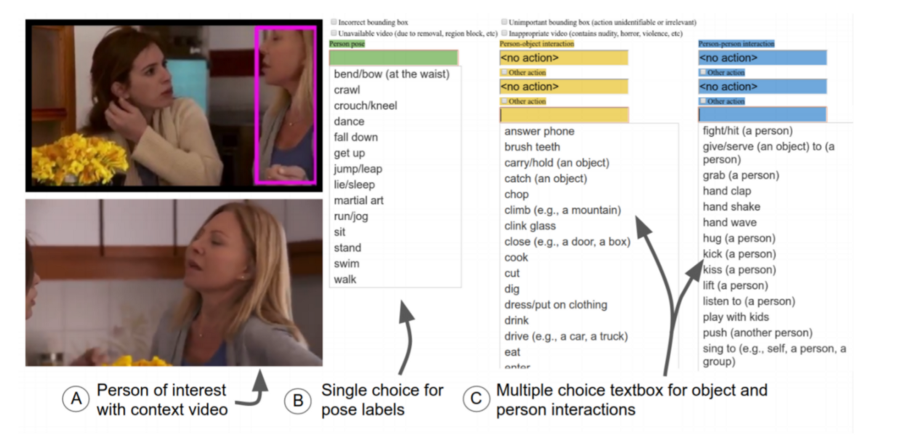
\includegraphics[width=1\textwidth]{chapter2/images/vocab.png}
		\caption{แสดง interface สำหรับสร้าง action label}
    	\label{fig:vocab}
\end{figure}
การสร้าง action labels จะถูกสร้างจากเหล่าคนที่เป็น annotators ซึ่งจะใช้ interface ในการสร้าง ซึ่งใน 1 กรอบสี่เหลี่ยม (bounding box) สามารถมี action labels ได้สูงสุดถึง 7 labels นอกจากนั้นสามารถตั้งสถานะบล็อก content ที่ไม่เหมาะสม หรือกรอบสี่เหลี่ยมที่ผิดพลาด (incorrect bounding box) ได้อีกด้วย ในทางปฎิบัติจะสังเกตได้ว่ามันมีโอกาศผิดอย่างหลีกเลี่ยงไม่ได้ เมื่อต้องได้รับคำสั่งให้หา action labels ที่ถูกต้องจาก 80 class จึงแบ่งขั้นตอนออกเป็น 2 ขั้นตอน คือ
\begin{enumerate}
	\item Action proposal  สอบถามเหล่า annotator เพื่อสร้างข้อเสนอสำหรับ action labels จากนั้นจับกลุ่มเข้าด้วยกัน ซึ่งจะทำให้มีโอกาสถูกต้องมากกว่าเป็นข้อเสนอแยกเดี่ยว
	\setlength\itemsep{-0.25em}
	\item Verification annotator จะตรวจสอบข้อเสนอที่ได้จากขั้นตอนแรก ซึ่งในแต่ละวิดิโอคลิปจะใช้มนุษย์ในการตรวจสอบ 3 คน เมื่อ action label ถูก annotator อย่างน้อย 2 คน ตรวจสอบ action label นั้นจะถูกยึดเป็นคำอธิบายหลัก
\end{enumerate}
\clearpage
\subsubsection*{3.การทดลองและวิเคราะห์ผล}	
\begin{figure}[!ht]
	\centering
	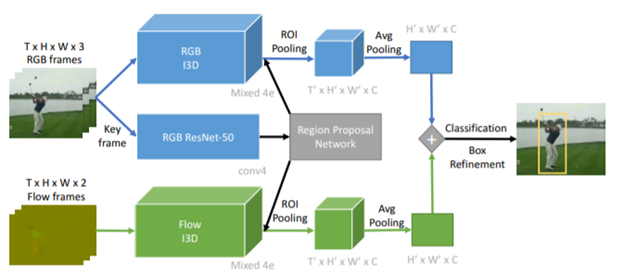
\includegraphics[width=1\textwidth]{chapter2/images/structure_ava.png}
		\caption{แสดง interface สำหรับสร้าง action label}
    	\label{fig:structure_ava}
\end{figure}
สำหรับโมเดลที่บทความ[2]นี้พูดถึงคือ two stream variant ซึ่งจะทำการประมวลผลทั้ง RGB flow และ optical flow และ เป็นโครงสร้างของ Faster RCNN ที่นำ Inception network เข้ามาใช้ 
\begin{enumerate}
	\item การทดลองที่ 1 ทดสอบว่าโมเดลใดให้ประสิทธิภาพการทำงานได้ดีที่สุด
	\begin{enumerate}
		\item รายละเอียดการทดลอง : นำชุดข้อมูล JHMDB และ UCF 101 มาเป็นชุดข้อมูลในการทดสอบ ซึ่งการทดลองจะทดสอบด้วย frame level และ video level และมี metrics ในการวัด คือ ใช้ค่า IOU (intersection over union)
		\item สำหรับ video level จะคำนวณ 3D IOUs ซึ่งเป็นการเปรียบเทียบระหว่าง ground truth tubes และ linked detection tubes (ground truth tube คือ การนำเอากรอบสี่เหลี่ยม (bounding box) จริงของวัตถุในเฟรมที่ติดต่อกันมาเรียงต่อกันเป็น tube และ linkded detection tube คือ การนำเอากรอบสี่เหลี่ยม (bounding box) ที่ตรวจเจอมาเรียงต่อกันเป็น tube)โดยตั้งค่าเกณฑ์ (threshold) ที่ 0.5 และรายงานผลออกเป็น mean average precision
	\begin{table}[!ht]
	\centering
	\begin{tabular}{|c|c|c|c|}
			\hline
			{Frame-mAP}&{JHMDB}&{UCF101-24}\\
			\hline
			Actionness 			& 39.9		& 	-						\\
			Peng w/o MR			& 56.9		& 64.8						\\
			Peng w/  MR 			& 58.5		& 65.7						\\
			ACT					& 65.7		& 69.5						\\
			\hline
			Out approach			& 73.3		& 76.3						\\
			\hline
		\end{tabular}
		\caption{ผลการทดลองของวิธีต่างๆบน Frame Level}
		\label{tab: transfer learning}
	\end{table}
	\begin{table}[!ht]
	\centering
	\begin{tabular}{|c|c|c|c|}
			\hline
			{Video-mAP}&{JHMDB}&{UCF101-24}\\
			\hline
			Peng w/ MR 			& 73.1		& 35.9						\\
			Singh				& 72.0		& 46.3						\\
			ACT			 		& 73.7		& 51.4						\\
			TCNN				& 76.9		& 	-						\\
			\hline
			Out approach			& 78.6		& 59.9						\\
			\hline
		\end{tabular}
		\caption{ผลการทดลองของวิธีต่างๆบน Video Level}
		\label{tab: transfer learning}
	\end{table}
		\item ผลการทดลองของ frame level ส่วนตารางด้านล่าง คือ video level ซึ่งผลการทดลองได้ผลลัพธ์ คือ วิธี two stream ได้ค่า mAP มากกว่า วิธีการอื่นๆ ทั้ง frame level , video level 
	\end{enumerate}
	\item การทดลองที่ 2 นำโมเดล 2 stream มาทดลองกับชุดข้อมูล AVA ซึ่งได้ผลลัพธ์ดังนี้
	\begin{table}[!ht]
	\centering
	\begin{tabular}{|c|c|c|c|c|}
			\hline
			{Model}&{Temp + Mode}&{JHMDB}&{UCF101-24}&{AVA}\\
			\hline
			2D		& 1   RGB + 5  Flow		& 52.1		& 60.1		& 13.7		\\
			3D		& 5   RGB + 5  Flow		& 67.9		& 76.1		& 13.6		\\
			3D 		& 10 RGB + 10 Flow		& 73.4		& 78.0		& 14.6		\\
			3D		& 20 RGB + 20 Flow		& 76.4		& 78.3		& 15.2		\\
			3D		& 40 RGB + 40 Flow		& 76.7		& 76.0		& 15.6		\\
			3D		& 50 RGB + 50 Flow		& 	-		& 73.2		& 15.5		\\
			\hline
			3D		& 20 RGB				& 73.2		& 77.0		& 14.5		\\
			3D		& 20 Flow				& 67.0		& 71.3		& 9.9		\\
			\hline
		\end{tabular}
		\caption{ประสิทธิภาพของโมเดลเมื่อถูก transfer learning ด้วยชุดข้อมูล ActivityNet โดยใช้ video-level presentation}
		\label{tab: transfer learning ActivityNet}
	\end{table}
	\begin{enumerate}
		\item ผลการทดลองของ frame level ส่วนตารางด้านล่าง คือ video level ซึ่งผลการทดลองได้ผลลัพธ์ คือ วิธี two stream ได้ค่า mAP มากกว่า วิธีการอื่นๆ ทั้ง frame level , video level 
	\end{enumerate}
\end{enumerate}
\subsubsection*{4.สรุปผลการทดลอง}	
\begin{enumerate}
	\item สำหรับโมเดล 2 stream ที่เป็น 3D จะได้ประสิทธิภาพมากกว่า 2D
	\item สำหรับ AVA 3D โมเดลจะทำงานได้ดีหลังจากผ่านไปมากกว่า 10 เฟรม
	\item จะทำให้สังเกตได้ถึงการเพิ่มขึ้นของความยาวของ temporal window
	\item การนำ RGB , optical flow มารวมกันจะทำงานได้มีประสิทธิภาพมากกว่ากว่าแยก input
	\item JHMDB และ UCF101–24 ผลการทำงานจะ saturate ที่ 20 เฟรม
\end{enumerate}
